\begin{tikzpicture}

%A matrix
\draw [fill=cyan, opacity=.2,rotate=90, thick]  (0.1,4.35) node (v1) {} rectangle (3.9,-3.75) node (v2) {};
\draw [thick,rotate=90,red] (v1) rectangle (3.9,3.1);
\draw [thick,rotate=90,red] (0.1,3.1) rectangle (3.9,1.8) node (v7) {};
\draw [thick,rotate=90,red] (0.1,-2.45) node (v6) {} rectangle (v2);
\draw[thick,red]  (v6) rectangle (1.15,3.9);
\draw[thick,red]  (v7) rectangle (-0.55,0.1);





\node at (-0.45,-1.4) {\huge \color{red} $ \underset{ \color{blue} ( Parity  \ checks)}{H_{ m \times n} }$};

% X vector
\draw [ thick] (5.85,5) rectangle (6.85,6);
\draw [thick] (6.85,5) rectangle (5.85,4);
\draw [thick] (5.85,4) rectangle (6.85,3);
\draw [] (5.85,3) node (v4) {} rectangle (6.85,-0.1) node (v5) {};
\draw [thick] (5.85,-0.1) rectangle (6.85,-1.1);
\draw [thick] (5.85,-1.1) rectangle (6.85,-2.1) node (v8) {};
\node at (6.45,-3.4) {\huge \color{red}  $\underset{\tiny \color{blue} (code \ vector)}{c_{n \times 1 }} $};
\node at (6.35,1.6) {\Large \bf \vdots};

\draw [thick] (v4) rectangle (6.85,2.1);
\draw [thick] (v5) rectangle (5.85,0.8);

% delta-x vector
\draw [ thick] (9.4,5) rectangle (10.4,6);
\draw [thick] (10.4,5) rectangle (9.4,4);
\draw [thick, fill=green] (9.4,4) rectangle (10.4,3);
\draw [] (9.4,3) node (v4) {} rectangle (10.4,-0.1) node (v5) {};
\draw [thick] (9.4,-0.1) rectangle (10.4,-1.1);
\draw [thick] (9.4,-1.1) rectangle (10.4,-2.1);
\node at (10,-3.4) {\huge \color{red}  $\underset{\color{black}}{\underset{\tiny \color{blue} (error \ vector)}{e}} $};
\node at (9.9,1.6) {\Large \bf \vdots};
\node at (4.8,2.1) {\bf \Huge $\times$};
\draw [thick] (v4) rectangle (10.4,2.1);
\draw [thick] (v5) rectangle (9.4,0.8);

\node at (8.2,2) {\Huge \bf $+$};


\node at (9.9,3.5) {\color{red} \huge $ e_i$};


% y







\node at (15.9,1.6) {\bf \vdots};

\node at (11.8,2) {\Huge = };
\node at (15.8,-0.75) {\color{red} \huge $y_{m \times 1} = e_i\underline{h}_i$};
\node [align=left, text width =3.5cm] at (16.5,-1.65) {\Large  \color{blue} (Syndrome)};

\node at (0.3,2.45) {\Huge \bf $\cdots$};



% b_k

\draw [thick] (15.4,4.1) node (v3) {} rectangle (16.4,3.1);
\draw [thick] (15.4,3.1) rectangle (16.4,2.1);
\draw [thick] (15.4,2.1) rectangle (16.4,1);
\draw [thick] (15.4,1) rectangle (16.4,0);
\draw[fill=red, opacity=0.2]  (v3) rectangle (16.4,0);
\node at (-1.35,1.6) { \color{blue}\Large  \bf  \vdots};









\draw [dashed,blue] (-4.35,3.9) rectangle (3.75,3);
\draw [dashed,blue] (-4.35,3) rectangle (3.75,2);
\draw[dashed,blue]  (v1) rectangle (3.75,1);
\node at (-3.85,4.5) {\huge \bf  \color{red} $h_0$};
\node at (-2.4,4.5) {\huge \bf \color{red} $h_1$};
\node at (-1.25,4.5) {\huge \bf  \color{red} $h_k$};
\node at (0.25,4.5) {\huge \bf  \color{red} $\cdots$};
\node at (1.8,4.5) {\huge \bf  \color{red} $h_{n-1}$};
\node at (3.15,4.5) {\huge \bf  \color{red} $h_n$};


\node at (9.9,4.55) {\large \bf \vdots};


\node at (13.45,2) {\bf \Huge $0$};
\node at (14.45,2) {\huge \bf +};

\draw [fill=orange, opacity=0.5] (v8) rectangle (5.85,6);


\end{tikzpicture}